% This is samplepaper.tex, a sample chapter demonstrating the
% LLNCS macro package for Springer Computer Science proceedings;
% Version 2.20 of 2017/10/04
%
\documentclass[runningheads]{llncs}
%
\usepackage{graphicx}
% Used for displaying a sample figure. If possible, figure files should
% be included in EPS format.
%
% If you use the hyperref package, please uncomment the following line
% to display URLs in blue roman font according to Springer's eBook style:
% \renewcommand\UrlFont{\color{blue}\rmfamily}

\begin{document}
%
\title{Simplex vs. Montecarlo, a brief comparision.\thanks{Supported by Universidad Tecnológica de Pereira.}}
%
%\titlerunning{Abbreviated paper title}
% If the paper title is too long for the running head, you can set
% an abbreviated paper title here
%
\author{Oscar Eduardo Bernal}
%
\authorrunning{O. Bernal}
% First names are abbreviated in the running head.
% If there are more than two authors, 'et al.' is used.
%
\institute{Universidad Tecnológia de Pereira, Colombia
\email{}}
%
\maketitle              % typeset the header of the contribution
%
\begin{abstract}
The Monte Carlo Method give us a process to solve big problems using randomness, by other side simplex is a method to solve linear optimization ploblems through an iterative process. Using HPC we can have an approach to parallel computing with a good amount of threads, but the Simplex method can't be easily parallelizable because in each iteration it depends of the previous state, while using Monte Carlo each step of the process is completely independient. Even so the question arises, is there really a difference between the Simplex method and the Monte Carlo method in a high-performance environment to solve linear optimization ploblems?

\keywords{HPC \and linear optimization \and Monte Carlo \and parallel computing \and Simplex}
\end{abstract}
%
%
%
\section{Introduction}
Es facil pensar en que un algoritmo puede ser mejor que otro, en especial cuando se trata de hacer tareas en paralelo, pero para poder lograr una comprension real de las implicaciones de una afirmación como esta se requiere, no solo un entendimiento de los algoritmos, si no tambien realizar un proceso de experimentacion, donde se pueda comprobar con datos reales la hipotesis planteada.

\subsection{Linear Optimization}
description of the problems

\subsection{Simplex Method}
method description

\subsection{Monte Carlo Method}
method description

\subsection{Parallel computing}
what is this?

\subsection{Hipotesis}
Teniendo en cuenta la informacion sobre los dos metodos que se abordan en este documento se plantea la siguient hipotesis: 
Montecarlo es mejor que el metodo Simplex para solucionar problemas de Optimizacion Lineales con un gran numero de variables.

\section{Implementation}
Para poder poner a prueba esta hipotesis se desarrollaron 3 implementaciones, la primera y mas basica es una implementacion secuencial del metodo simplex, la segunda es una implementacion lineal del metodo montecarlo, y la ultima una version concurrente del metodo montecarlo.

\subsection{Sequential Simplex Method}
El metodo Simplex parte de una matriz nxm donde n es el numero de variables del problema y m es el numero de restricciones, sobre esta matriz se empieza a iterar cambiando los valores de ciertas filas y columnas en cada iteracion, hasta que se encuentra la solucion.
Este metodo tiene una complejidad algoritmica de orden cuadrado O(n2)­ en el peor de los casos, y en el mejor una complejidad de orden lineal (n+m)

\subsection{Sequential Monte Carlo Method}
El metodo Monte Carlo en su version secuencial realiza un numero fijo de pasos, que para este estudio es de 21.474.836, en los cuales genera n numeros aleatorios y luego realiza m+1 validaciones (siendo n y m el numero de variables y de restricciones respectivamente), para determinar si estos numeros cumplen con las condiciones del algoritmo, este ciclo se realiza multiples veces, obteniendo cada vez distintos valores guardando unicamente el estado para el cual el problema de optimizacion lineal es maximo.
Este metodo tiene una complejidad algoritmica de orden lineal O(n) en cualquier caso, ya que sin importar el resultado el se ejecuta un numero fija de veces, que no aumenta ni disminuye. 

\subsection{Parallel Monte Carlo Method}
La implementacion paralela del metodo de Monte Carlo crea una cantidad fija de hilos en cada bloque, que para este caso son 1024, y una rejilla de 1024 bloques, se utiliza una estructura lineal tanto para la distribucion de la rejilla asi como para la del bloque, para facilitar la comprension del algoritmo, pero esta se puede ampliar a una estructura tridimensional sin mayor problema.
\paragraph{}
El Kernel de este metodo se comporta de forma similar a su predecesor secuancial, probando distintas combinaciones de numeros aleatorios, y guardando en una matriz el estado del minimo encontrado, para luego de forma secuencial recorrer esta matriz para encontrar el valor minimo de todos, este recorrido no se hace de la totalidad de la matriz, si no de una sola posicion de la matriz, quedando de esta forma con complejidad lineal para el Kernel y lineal tambien para la determinacion del menor.

\section{Results}
Luego de ejecutar los metodos implementados para problemas de optimizacion con diferentes numeros de variables y restricciones, se encontro que los tiempos de ejecucion no resultaron como se esperaba, aunque el comportamiento de los algoritmos corresponde con el orden de complejidad, la magnitud de los tiempos demuestra la importancia de la experimentacion.
\paragraph{}
Asi se tiene que aunque el metodo Simplex tiene una complejidad de orden cuadrado, esto es unicamente en el peor de los casos y este es un caso extraño, ya que en la mayoria de problemas el caso mas comun es de orden lineal, causando asi tiempos de ejecucion menores que la ejecucion de Monte Carlo, que se comporta igualmente con orden lineal pero con un tiempo inicial mayor.

\begin{figure}
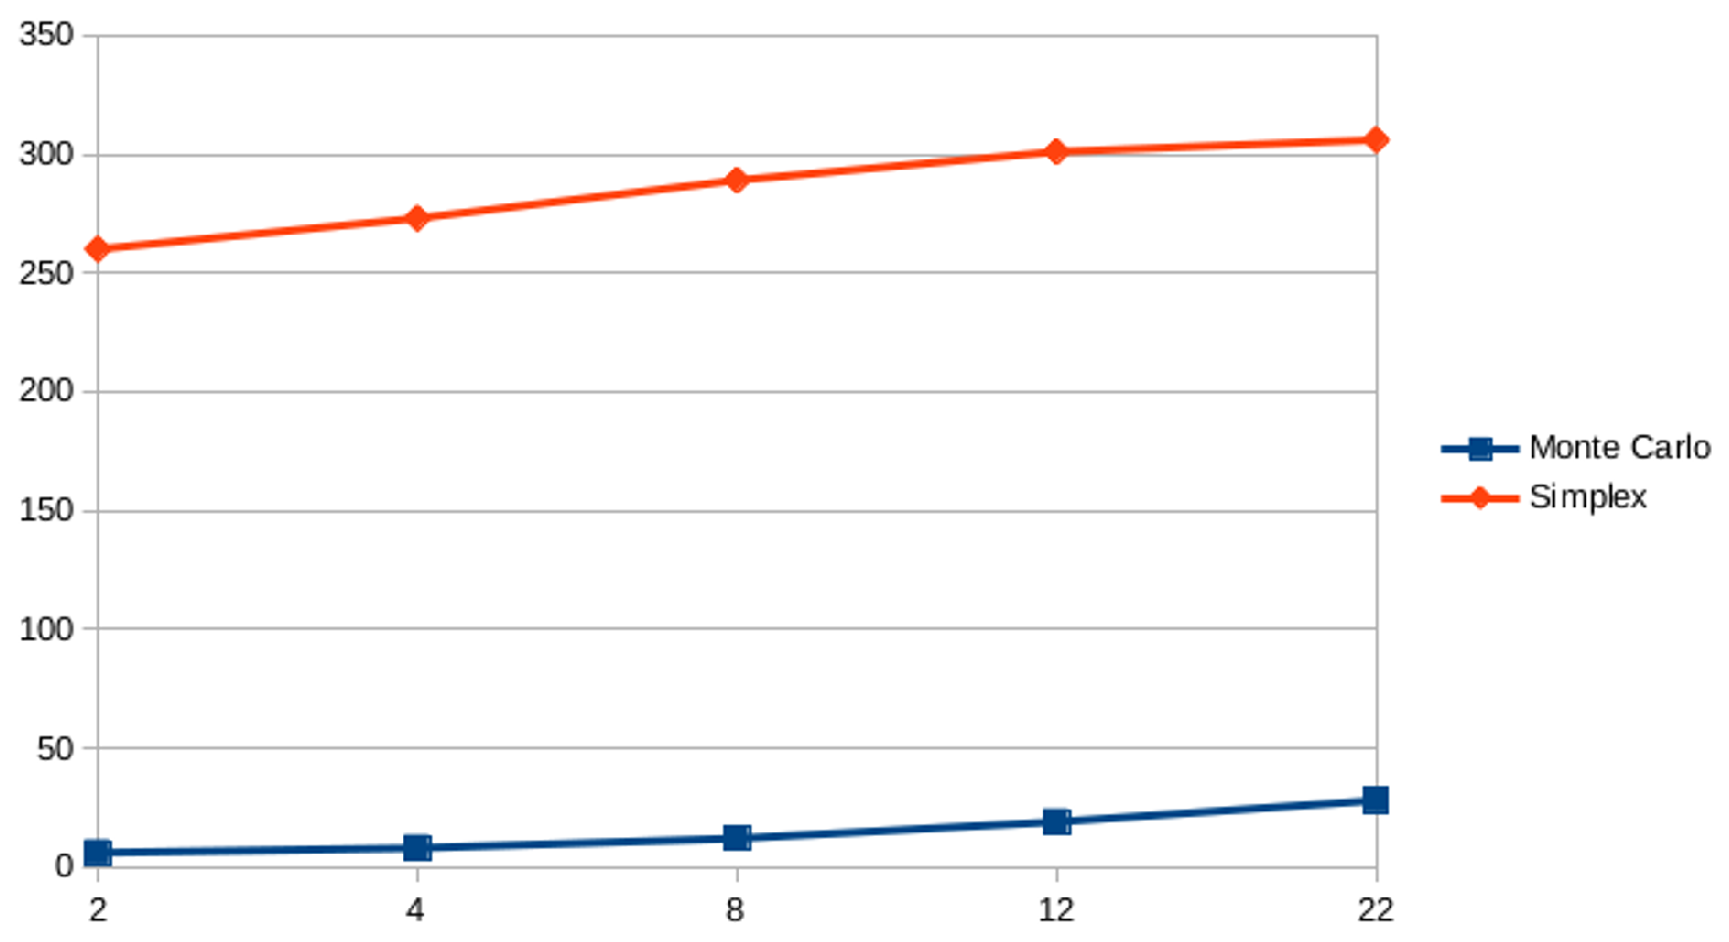
\includegraphics[width=\textwidth]{fig1.eps}
\caption{A figure caption is always placed below the illustration.
Please note that short captions are centered, while long ones are
justified by the macro package automatically.} \label{fig1}
\end{figure}

\section{Conclusions}
put here something to say

no siempre paralelo es mejor, 

%
% ---- Bibliography ----
%
% BibTeX users should specify bibliography style 'splncs04'.
% References will then be sorted and formatted in the correct style.
%
% \bibliographystyle{splncs04}
% \bibliography{mybibliography}
%
\begin{thebibliography}{8}
\bibitem{ref_article1}
Author, F.: Article title. Journal \textbf{2}(5), 99--110 (2016)

\bibitem{ref_lncs1}
Author, F., Author, S.: Title of a proceedings paper. In: Editor,
F., Editor, S. (eds.) CONFERENCE 2016, LNCS, vol. 9999, pp. 1--13.
Springer, Heidelberg (2016). \doi{10.10007/1234567890}

\bibitem{ref_book1}
Author, F., Author, S., Author, T.: Book title. 2nd edn. Publisher,
Location (1999)

\bibitem{ref_proc1}
Author, A.-B.: Contribution title. In: 9th International Proceedings
on Proceedings, pp. 1--2. Publisher, Location (2010)

\bibitem{ref_url1}
LNCS Homepage, \url{http://www.springer.com/lncs}. Last accessed 4
Oct 2017
\end{thebibliography}
\end{document}
